\subsection{Supporting Pattern}

Entwurfsmuster und Architekturmuster sind zwei wichtige Konzepte in der Softwareentwicklung, die dazu beitragen, wiederverwendbare Lösungen für wiederkehrende Probleme zu finden. Sie unterscheiden sich hauptsächlich in ihrem Anwendungsbereich und ihrer Abstraktionsebene~\cite{gamma1994design}.
\\\\
Entwurfsmuster sind wiederverwendbare Lösungen für häufig auftretende Probleme auf der Ebene von Klassen und Objekten. In der deutschen Sprache setzt sich auch häufig der englische Begriff Patterns durch. Sie sind in der Regel kleiner und detaillierter als Architekturmuster und bieten Best Practices für bestimmte Designprobleme. Entwurfsmuster sind in der Regel unabhängig von einer bestimmten Programmiersprache und können in verschiedenen Projekten und Systemen eingesetzt werden.
\\\\
Einige bekannte Entwurfsmuster, die auch für verteilte Systeme und in diesem Skript eine Rolle spielen sind:
\begin{itemize}
\item \textbf{Singleton}: Stellt sicher, dass eine Klasse nur \textbf{eine} Objektinstanz hat und stellt einen globalen Zugriffspunkt dafür bereit. Beispiel: Eine zentrale Konfigurationsklasse, die von verschiedenen Teilen einer Anwendung gemeinsam genutzt wird.
\item \textbf{Observer}: Ermöglicht einem Objekt (Subject), seinen Zustand automatisch an abhängige Objekte (Observer) zu übermitteln, wenn Änderungen eintreten. Beispiel: Ein Event-Listener-System, das Benachrichtigungen an Abonnenten sendet, wenn bestimmte Ereignisse eintreten.
\item \textbf{Factory Method}: Definiert eine Schnittstelle zum Erstellen von Objekten in einer Superklasse, während Unterklassen die genaue Klasse der zu erzeugenden Objekte bestimmen. Beispiel: Ein Framework für die Erstellung verschiedener Arten von Diagrammen, bei dem jede Diagrammklasse ihre eigenen Erstellungsregeln hat.
\item \textbf{Adapter}: Ermöglicht es, die Schnittstelle einer bestehenden Klasse so anzupassen, dass sie mit einer anderen Klasse kompatibel ist, ohne den Quellcode der beiden Klassen zu ändern. Beispiel: Eine Anwendung, die verschiedene Zahlungsschnittstellen unterstützt, verwendet Adapter, um die unterschiedlichen Schnittstellen in eine einheitliche API umzuwandeln.
\end{itemize}
Architekturmuster sind wiederum Best Practices für den Entwurf der Gesamtstruktur einer Softwareanwendung oder eines Systems. Sie befassen sich mit der Organisation von Code, Komponenten und deren Kommunikation auf einer höheren Abstraktionsebene. Architekturmuster bieten Lösungen für übergreifende Anliegen wie Skalierbarkeit, Flexibilität, Wartbarkeit und Testbarkeit.
\\\\
Einige bekannte Architekturmuster sind:
\begin{itemize}
\item \textbf{Schichtenarchitektur} (Layered Architecture): Das Architekturmuster unterteilt eine Anwendung in Schichten, wobei jede Schicht eine bestimmte Funktion hat, wie z.B. Präsentation, Geschäftslogik oder Datenzugriff. Dies ist sehr stark verbunden mit der Zerlegung des Teilproblems.
\item \textbf{Model-View-Controller} (MVC): Trennt eine Anwendung in drei Hauptkomponenten - das Modell (Daten und Geschäftslogik), die Ansicht (Präsentation und Benutzerinteraktion) und den Controller (Steuerung der Datenverarbeitung und Aktualisierung der Ansicht). Beispiel: Ein Content-Management-System, das Daten speichert, Benutzerinhalte anzeigt und Benutzeraktionen verarbeitet.
\end{itemize}
Um beispielhaft die Bedeutung und die Anwendung des MVC-Musters deutlich zu machen, soll ein Fallbeispiel erarbeitet werden, das dieses Muster verwendet. Es ist zwar möglich, das Beispiel auch mit anderen bekannten Architekturmuster umzusetzen, jedoch liegt hier nicht der Fokus. Es soll aber vor der Diskussion kurz darauf hingewiesen werden, dass sich in der Praxis  weitere Begriffe wie das Model-View-Presenter-, das Model-View-ViewModel- oder das Model-View-Adapter-Muster oder auch weit komplexere Ansätze etabliert haben. Alle gemein haben sie, dass sie versuchen, spezifische Varianten des MVC-Musters genauer zu beschreiben.

\subsubsection{Model Viewer Controller}
Zunächst konzentrieren wir uns auf die wesentlichsten Eigenschaften des MVC Patterns. Die erste ist im Zweifel direkt eine eher verwirrende. Das MVC-Pattern kann sowohl ein Entwufsmuster, also ein grober Designentwurf sein, als auch ein Architekturpattern mit einem konkreten Vorschlag der Implementierung. Wichtig festzustellen ist, auch wenn man andere Quellen zur Recherche nutzt, auf welcher Ebene das Pattern adressiert wird.  Hier konzentriert sich diese Ausführung im weiteren auf das MVC-Architekturmuster, da die Diskussion des MVC-Entwurfsmusters im grundlegenden Ansatz bereits bei der Unterscheidung von Schichten und Tiers erörtert wurde. Das MVC-Entwurfsmuster kann aus der Tier Diskussion als Three-Tier-Architektur Entwurf verstanden werden und braucht daher für das grundlegende Verständnis keine weitere Erklärung.
\\\\
In dem Diagramm~\ref{fig:default-mvc} repräsentieren die Klassen Model, View und Controller die drei Hauptkomponenten des MVC-Architekturmusters:
\begin{itemize}
\item \textbf{Model} (Modell): Kapselt Daten und Geschäftslogik. Es enthält Methoden, um Beobachter hinzuzufügen, zu entfernen und zu benachrichtigen.
\item \textbf{View} (Ansicht): Implementiert meist das Observer-Interface und ist für die Präsentation und Benutzerinteraktion verantwortlich. Die \enquote{update()} Methode wird aufgerufen, wenn das Modell Änderungen benachrichtigt.
\item \textbf{Controller} (Controller): Steuert die Datenverarbeitung und aktualisiert die Ansicht basierend auf Benutzeraktionen und Modelländerungen.
\end{itemize}

\begin{figure}[ht]
  \centering
  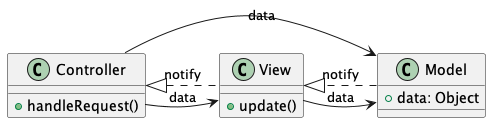
\includegraphics[width=0.8\textwidth]{fig/uml/default-mvc.png}
  \caption{Beispiel eines Basis MVC Architekturmusters}
  \label{fig:default-mvc}
\end{figure}

Diese Basisarchitektur wird nun in ein Fallbeispiel überführt, um verschiedene Aspekte zu diskutieren. Das Szenario für die Fallstudie soll eine einfache Led-Lampe sein, die über eine eigene CPU und eigenen Speicher und einen Bluetooth Sender und Empfänger verfügt. Der Aufbau ist erweitert durch einen Raspberry PI, der sowohl die Anbindung der Lampe über Bluetooth repräsentiert, als auch den Servicezugriffspunkt für Applikationen im Internet. Der Raspberry Pi kann über eine Global Unicast IPv6 Adresse erreicht werden, um Steuerungssignale für die Lampe über die App abzugeben. 

Wir nutzen daher das Architekturmuster um eine Aufteilung in Verantwortlichkeiten zu realisieren. Jede Verantwortlichkeit - des PI, der Lampe und der Nutzerapp - wird in einer Klasse gekapselt. Die Zugehörigkeit zum MVC Pattern wird in diesem Beispiel dadurch Stereotypen zum Ausdruck gebracht.
\\\\
Eine Stereotype ist eine benutzerdefinierte Kennzeichnung eines UML-Elements, die durch das Hinzufügen von Namen, Attributen und Methoden definiert werden kann. Sie erweitern die UML-Notation und ermöglichen es, zusätzliche Informationen oder Bedeutungen einem Element zuzuweisen, ohne die zugrunde liegende UML-Syntax zu ändern. Stereotypen können auch dazu verwendet werden, bestimmte Funktionen oder Verhaltensweisen hinzuzufügen, die von der Basis-UML-Syntax nicht unterstützt werden. Zum Beispiel kann eine Stereotype \enquote{Singleton} einem Klassenobjekt hinzugefügt werden, um anzuzeigen, dass nur eine einzige Instanz dieser Klasse im gesamten System vorhanden sein sollte, oder wie in diesem Fall die Sterotype  \enquote{Model}. Mit Model wird die Klasse Lampe mit der Aufgabe des Buisnessmodells gebunden. 
Die Abbildung~\ref{fig:stereo-mvc} zeigt das sich nun ergebene Bild. 
\begin{figure}[ht]
  \centering
  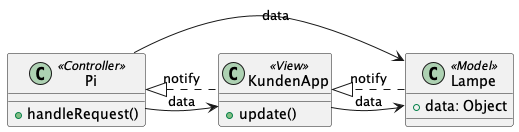
\includegraphics[width=0.8\textwidth]{fig/uml/sterotypen-mvc.png}
  \caption{MVC Architekturmusters im Fallbeispiel mit Sterotypen}
  \label{fig:stereo-mvc}
\end{figure}

Die Aufgaben der einzelnen Komponenten eines MVC-Architekturpatterns sind aber nicht trennscharf und sind wirklich einzig als ein \enquote{Best Practise} Beispiel anzusehen. Die folgende Aufzählung soll nur ein Einblick darin geben, wie weit die Aufgabenfelder der Komponenten erweitert werden, können ohne das MVC-Architekturpattern zu verletzen. 
\begin{itemize}
\item Eine MVC-View kann neben ihrer Hauptfunktion, der Präsentation von Daten, auch weitere Aufgaben übernehmen. Sie kann beispielsweise automatisch die Darstellung von Daten anpassen, wenn Änderungen in den zugehörigen Modellen der Anwendung vorgenommen werden. Zudem kann sie Benutzeraktionen, die über grafische Eingabeelemente wie Textfelder oder Buttons erfolgen, an den Controller weiterleiten. Zusätzlich ist es möglich, dass die View Status- und Fehlermeldungen von Controllern visualisiert.

\item Ein MVC-Controller kann zusätzlich zu seiner Hauptaufgabe, der Steuerung des Datenflusses, weitere Funktionen übernehmen. Er kann beispielsweise Systemsignale wie eine Systemuhr verarbeiten und entsprechend darauf reagieren (z.B. Budget reicht nicht mehr für Nutzung). Zudem kann er die Komponentenlogik der Anwendung umsetzen und die Kommunikation mit externen Datenquellen für den Zweck der Datensynchronisation übernehmen.

\item Ein MVC-Modell kann neben der zentralen Verwaltung von Daten auch anderen Modulen Zugriff auf die Zustandsdaten gewähren und diese über Änderungen informieren, in der Regel mithilfe des Observer-Patterns. Zudem kann es die Komponentenlogik der Anwendung umsetzen und die Kommunikation mit externen Datenquellen koordinieren.
\end{itemize}

\subsubsection{VCM und CVM}
Das MVC Pattern selbst kann auch in unterschiedlichen Schichtenmodellen gedacht werden und in ihrer Ausprägung beispielhaft als VCM und CVM bezeichnet werden.  Es ist wichtig zu beachten, dass VCM und CVM für sich keine weit verbreiteten oder standardisierten Architekturmuster sind und eher als Variationen des MVC-Musters betrachtet werden sollten. Bei den Variationen werden die Reihenfolge der Komponenten verändert und je mit einem Schichtenmodell vereint. Die Abbildung~\ref{fig:mvs-varianten} soll je Ausprägung eine mögliche Interpretation verdeutlichen.

\begin{figure}[ht]
  \centering
  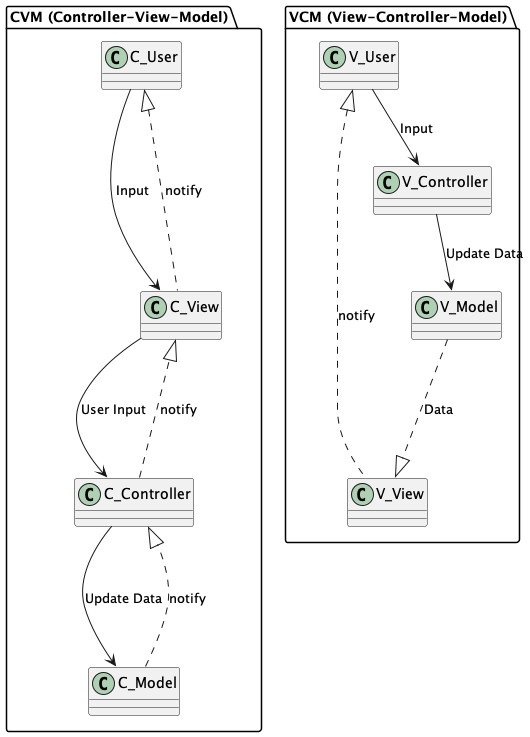
\includegraphics[width=0.65\textwidth]{fig/uml/mvc-varianten.png}
  \caption{Mögliche Varianten vom MVC in Schichten gedacht}
  \label{fig:mvs-varianten}
\end{figure}
Die drei Module einer Model-View-Controller (MVC)-Komponente sind gemäß dem Schichtenparadigma in Ebenen angeordnet. Die höheren Ebenen können auf die tiefergelegenen Ebenen zugreifen, aber nicht umgekehrt. Dies entspricht den Anforderungen an ein gerichtetes Schichtenmodel. 
\\\\
Die unterste Ebene enthält das Modell. Das zugehörige Modul weiß nichts von den über ihm liegenden Modulen und kann mit diesen nur indirekt\footnote{zum Beispiel durch Antworten auf Nachrichten oder mit Hilfe eines sogenannten \enquote{handle} oder \enquote{callback}} kommunizieren.
\\\\
Ein Controllermodul kann direkt auf ein Modellmodul zugreifen, um die Inhalte zu manipulieren. Eine View kommuniziert im Allgemeinen nur direkt mit Controllermodulen, um diesen Benutzeraktionen mitzuteilen.
\\\\
In dem hier vorgestellten Szenario stellt der Benutzer das „oberste Modul“ dar. Es kommuniziert nur gerichtet mit den View- und Controllermodulen. 
\\\\
Wo die in diesem Beispiel aufgebaute CVM Struktur alle Schichten für den Weg zum Modell benutzt und mit dem \enquote{handle} über die Auswirkungen informiert, wird im Beispiel des VCM Model für den Input die Schicht der View Klasse übersprungen, um eine direktere Eingabe zu unterstützen. Somit unterstützt die VCM Struktur das MVC Muster und das Schichtenmodell. Es eignet  sich aber auch für die Verarbeitung von zeitkritischen Inputs, wie sie beispielhaft in einem Jump'n'Run-Spiel gefordert sind. Der besonderer Nachteil ist, es braucht direkte Kommunikationskanäle. Dieser direkte Weg ist aber nicht immer möglich. Auch verlangen Technologien oder auch Frameworks bei User-Inputs nicht selten die klare Trennung von View und Controller. Ein Beispiel für solch eine technologische Anforderung wird von Java FX repräsentiert.     

\paragraph{Beispiel: JavaFX als\\\\}
JavaFX ist ein relativ modernes Framework zur Erstellung von graphischen Benutzeroberflächen (GUIs) in Java. Es bietet verbesserte Möglichkeiten im Vergleich zu AWT und Swing. In JavaFX werden Benutzereingaben (User Inputs) über das Event-Handling-System verarbeitet. Hier ist ein Überblick darüber, wie JavaFX mit Benutzereingaben umgeht:
\begin{itemize}
\item Event-Handling: In JavaFX werden Ereignisse (Events) verwendet, um Benutzereingaben wie Mausklicks, Tastaturanschläge und andere Aktionen zu verarbeiten. Jedes Steuerelement (Control) oder Node in JavaFX kann Event-Handler registrieren, um auf spezifische Ereignisse zu reagieren.
\item Event-Typen: JavaFX bietet verschiedene Event-Klassen, die unterschiedliche Arten von Benutzereingaben repräsentieren, z. B. MouseEvent, KeyEvent, ScrollEvent usw. Sie können Event-Handler erstellen, die auf bestimmte Event-Typen reagieren, indem Sie die entsprechenden Methoden überschreiben.
\item Event-Handler: Um auf ein Ereignis zu reagieren, müssen Sie einen Event-Handler erstellen, der eine Methode handle() implementiert, die den Ereignistyp als Parameter akzeptiert. Sie können einen Event-Handler entweder als separate Klasse oder als Lambda-Ausdruck erstellen.
 \end{itemize}   

Das Code-Listing~\ref{lst:javafx-input} macht diese Anforderung dadurch deutlich, das die Java FX Anwendung die \enquote{javafx.application.Application} ableitet. In diesem Beispiel wird ein einfacher Button erstellt, der auf Mausklicks reagiert. Der Event-Handler wird mithilfe eines Lambda-Ausdrucks definiert und beim Klicken des Buttons wird \enquote{Button clicked!} in der Konsole ausgegeben. An dieser Stelle könnten die Daten vom Nutzer auch an den Controller weitergegeben werden.

\subsubsection{Vertreter}
Auch für die Verteilten Systeme machen die Schnittstellen und die Zuordnungen einen wichtigen Unterschied. Jede Bindung der Komponenten bedarf einer Kommunikation, die im Zweifel mit einem Kommunikationsweg  verbunden ist. Dieser Anforderung muss das Overlay- wie auch das physikalische Netzwerk entsprechen. Dies kann weitreichende Entscheidungen mit sich bringen. Stellen wir uns vor, dass die Lampe in unserem Fallbeispiel über Bluetooth angesprochen werden muss, so ist aus der View kein direkter physikalischer Kommunikationsweg vorhanden, um einen \enquote{handle} zu nutzen ohne den Controller oder einen etwaigen Proxy einzusetzen.  Ein Proxy in einem verteilten System ist eine Komponente, die als Vermittler zwischen Clients und entfernten Diensten fungiert. 
\\\\
Der Proxy\index{Proxy} ist eine Art Stellvertreter für den entfernten Dienst und ermöglicht es dem Client, auf diesen Dienst zuzugreifen, als ob er sich lokal im selben Netzwerk befände.
Der Proxy wird typischerweise zwischen dem Consumer und dem entfernten Dienst (Provider) platziert und übernimmt die Verwaltung der Kommunikation zwischen diesen beiden Komponenten. Der Client sendet Anfragen an den Proxy, der die Anfrage entgegennimmt und an den entfernten Dienst weiterleitet. Der entfernte Dienst sendet die Antwort an den Proxy zurück, der die Antwort an den Client weiterleitet.\\\\

\noindent\begin{minipage}{\textwidth}
\begin{lstlisting}[caption={Java FX Input},captionpos=b,label={lst:javafx-input}]
import javafx.application.Application;
import javafx.scene.Scene;
import javafx.scene.control.Button;
import javafx.scene.layout.StackPane;
import javafx.stage.Stage;

public class JavaFXUserInputExample extends Application {

    public static void main(String[] args) {
        launch(args);
    }

    @Override
    public void start(Stage primaryStage) {
        Button button = new Button("Click me!");

        // Registering an EventHandler for the button click
        button.setOnAction(event -> {
            System.out.println("Button clicked!");
        });

        StackPane root = new StackPane();
        root.getChildren().add(button);

        Scene scene = new Scene(root, 300, 250);

        primaryStage.setTitle("JavaFX User Input Example");
        primaryStage.setScene(scene);
        primaryStage.show();
    }
}
\end{lstlisting}
\end{minipage}

Ein Proxy bietet mehrere Vorteile in einem verteilten System. Zum Beispiel kann ein Proxy mit Caching dazu beitragen, die Netzwerklatenz zu reduzieren, indem er Anfragen von Clients bündelt und sie in einer einzigen Anfrage an den entfernten Dienst weiterleitet. Ein Proxy kann auch die Sicherheit erhöhen, indem er den Zugriff auf den entfernten Dienst kontrolliert und Anfragen von unautorisierten Clients blockiert. Das Diagramm \ref{fig:proxy} beschreibt die Idee als Muster von Komponenten:
\begin{figure}[ht]
  \centering
  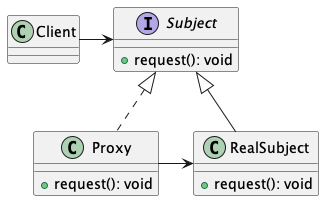
\includegraphics[width=0.45\textwidth]{fig/uml/proxy.png}
  \caption{Proxy Pattern}
  \label{fig:proxy}
\end{figure}
\begin{itemize}
\item \textbf{Client}: Die Klasse, die mit dem Subject-Interface interagiert.
\item \textbf{Subject}: Das Interface, das von Proxy und RealSubject implementiert wird. Es definiert die gemeinsame Schnittstelle für Proxy und RealSubject.
\item \textbf{RealSubject}: Die Klasse, die das eigentliche Objekt repräsentiert, auf das der Proxy zugreifen soll.
\item \textbf{Proxy}: Die Klasse, die den Zugriff auf das RealSubject steuert.
\end{itemize}

Der Client interagiert mit dem Subject-Interface und kennt nicht den Unterschied zwischen Proxy und RealSubject. Der Proxy implementiert das Subject-Interface und steuert den Zugriff auf das RealSubject.
\\\\
Es gibt verschiedene Arten von Proxies, die in einem verteilten System verwendet werden können, wie z.B. Forward Proxy, Reverse Proxy, Caching Proxy und Load Balancing Proxy. Jede Art von Proxy hat ihre eigenen Funktionen und Vorteile, je nach den Anforderungen des Systems und der Architektur:

\begin{itemize}
\item Ein \textbf{Forward Proxy} ist ein Proxy-Server, der als Vermittler zwischen einem Client und dem Internet fungiert. Wenn ein Client eine Anfrage an das Internet sendet, geht die Anfrage zuerst an den Forward Proxy-Server, der dann die Anfrage an das Ziel weiterleitet und die Antwort des Ziels an den Client zurücksendet.

Der Hauptzweck eines Forward Proxys besteht darin, die Privatsphäre und Sicherheit des Clients zu schützen, indem er seine Identität und IP-Adresse vor dem Zielserver verbirgt. Dadurch kann der Client anonym im Internet surfen und verhindern, dass die besuchten Websites seine IP-Adresse oder Identität aufzeichnen.

Forward Proxies werden auch oft in Unternehmen eingesetzt, um den Zugriff auf das Internet zu kontrollieren und zu beschränken. Sie können beispielsweise bestimmte Websites oder Dienste blockieren oder die Verwendung von bestimmten Protokollen einschränken.
\item Im Gegensatz zu einem Forward Proxy, der den Datenverkehr vom Client zu den Servern weiterleitet, empfängt ein \textbf{Reverse Proxy} Anfragen von den Servern und leitet sie an den Client weiter.

Der Hauptzweck eines Reverse Proxys besteht darin, die Last auf die Server zu verteilen, indem er eingehende Anfragen an verschiedene Server weiterleitet, um eine bessere Auslastung und Lastverteilung zu erreichen. Er kann auch zur Beschleunigung der Website-Leistung verwendet werden, indem er häufig angeforderte statische Inhalte im Cache speichert und schneller bereitstellt.

Reverse Proxies werden auch oft als Sicherheitsmaßnahme eingesetzt, um Angriffe auf die Server abzuwehren, indem sie den Server vor direktem Zugriff aus dem Internet schützen und nur autorisierte Anfragen durchlassen.

\item Ein \textbf{Caching Proxy} ist ein Proxy-Server, der den Datenverkehr zwischen einem Client und dem Internet überwacht und häufig abgerufene Inhalte im Cache speichert, um die Website-Leistung zu verbessern und die Belastung der Internetverbindung zu reduzieren.

Wenn ein Client eine Anfrage an das Internet sendet, überprüft der Caching Proxy, ob er eine Kopie der angeforderten Ressource im Cache hat. Wenn dies der Fall ist, wird die Ressource aus dem Cache geladen und an den Client zurückgesendet, ohne dass eine Verbindung zum ursprünglichen Server hergestellt werden muss. Wenn die Ressource nicht im Cache vorhanden ist, leitet der Caching-Proxy die Anfrage an den Server weiter und speichert dann die Antwort im Cache für zukünftige Anforderungen.

Caching-Proxies können dazu beitragen, die Leistung von Websites zu verbessern und die Latenzzeiten zu reduzieren, da häufig angeforderte Ressourcen schneller geladen werden können. Sie können auch dazu beitragen, die Bandbreitennutzung zu reduzieren, da der Proxy den Datenverkehr filtern und nur die notwendigen Ressourcen im Cache speichern kann.
\item Ein \textbf{Load Balancing Proxy} ist ein Proxy-Server, der als Vermittler zwischen einem Client und einem oder mehreren Servern fungiert und die Last auf mehrere Server verteilt, um eine bessere Auslastung und Verfügbarkeit zu erreichen.

Wenn ein Client eine Anfrage an den Load Balancing Proxy sendet, überprüft der Proxy die Server, die die Anfrage bearbeiten können, und leitet die Anfrage dann an den am wenigsten ausgelasteten Server weiter. Dadurch können mehrere Server gleichzeitig Anfragen bearbeiten, wodurch die Leistung und Verfügbarkeit der Anwendung verbessert werden.

Load Balancing Proxies sind besonders nützlich für Websites und Anwendungen mit hohem Traffic oder schweren Workloads, da sie dazu beitragen, die Belastung auf die Server zu reduzieren und eine hohe Verfügbarkeit sicherzustellen. Darüber hinaus können Load Balancing Proxies auch dazu beitragen, die Ausfallsicherheit zu verbessern, da im Falle eines Ausfalls eines Servers die Anfragen automatisch auf einen anderen Server umgeleitet werden können.
\end{itemize}
Ein Proxy ist normalerweise ein Vermittler, der  auf der Netzwerkebene arbeitet und als Gateway zwischen dem Client und dem Server fungiert. Eine Alternative Form zum Proxy kann auch als Broker beschrieben werden. 

Broker und Proxies sind beide Vermittler, die in der Kommunikation zwischen verschiedenen Anwendungen verwendet werden. Der Hauptunterschied zwischen den beiden besteht darin, wie sie diese Kommunikation verarbeiten und welche Funktionen sie bereitstellen.
\\\\
Ein \textbf{Broker} ist ein Vermittler, der die Kommunikation zwischen verschiedenen Anwendungen ermöglicht, indem er Nachrichten empfängt, speichert und an die richtigen Empfänger weiterleitet. Der Broker ist normalerweise in der Lage, die Nachrichten zu filtern, zu transformieren oder zu aggregieren, bevor er sie an den Empfänger weiterleitet. Der Broker kann auch verschiedene Messaging-Protokolle unterstützen und die Nachrichten in einer Warteschlange speichern, wenn der Empfänger nicht verfügbar ist. 

\begin{figure}[ht]
  \centering
  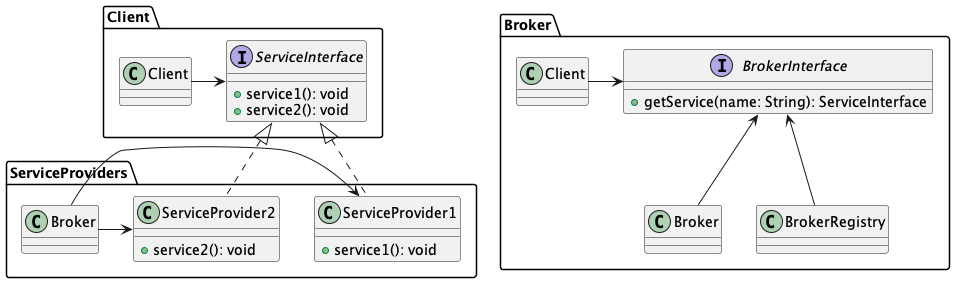
\includegraphics[width=0.95\textwidth]{fig/uml/broker.png}
  \caption{Broker Pattern}
  \label{fig:broker}
\end{figure}

Das Diagramm \ref{fig:broker} beschreibt das Broker-Pattern mit den folgenden Komponenten:
\begin{itemize}
\item \textbf{Client}: Die Klasse, die einen Dienst von einem der Service-Provider anfordert.
\item \textbf{ServiceInterface}: Das Interface, das von den ServiceProvidern implementiert wird. Es definiert die gemeinsame Schnittstelle für die angebotenen Dienste.
\item \textbf{ServiceProvider1, ServiceProvider2}: Die Klassen, die die tatsächlichen Dienste bereitstellen und das ServiceInterface implementieren.
\item BrokerInterface: Das Interface, das von Broker und BrokerRegistry implementiert wird. Es definiert die gemeinsame Schnittstelle, um auf die verschiedenen Dienste zuzugreifen.
\item \textbf{Broker}: Die Klasse, die als Vermittler zwischen Client und ServiceProvider fungiert und die Kommunikation vereinfacht.
\item \textbf{BrokerRegistry}: Die Klasse, die alle verfügbaren ServiceProvider verwaltet und dem Broker bei Bedarf zur Verfügung stellt.
\end{itemize}
Der Client greift über das BrokerInterface auf die gewünschten Dienste zu, ohne direkt mit den ServiceProvider-Klassen zu interagieren. Der Broker verwaltet die Kommunikation zwischen Client und ServiceProvider und entkoppelt so deren Abhängigkeiten.

Es ist weiter möglich eine weitere Unterschiedung in \textbf{Forwarding-Broker} und \textbf{Handle-Driven-Broker} einzuführen. 
\\\\
Ein Forwarding-Broker ist ein Broker, der eingehende Nachrichten an den Empfänger weiterleitet, der von der Nachrichtadresse identifiziert wird. Der Broker hat keine Vorstellung von der Struktur oder dem Inhalt der Nachrichten, sondern dient lediglich als Vermittler zwischen Sender und Empfänger. Es handelt sich um ein sehr einfaches System, das schnell und effizient arbeitet, aber nur minimale Unterstützung für die Transformation von Nachrichten bietet.
\\\\    
Ein Handle-Driven-Broker ist dagegen ein Broker, der Nachrichten auf Basis eines Handles weiterleitet, das als Referenz auf eine Nachricht dient. Der Broker speichert den \enquote{handle} und bietet verschiedene Funktionen an, um die Nachrichten zu bearbeiten oder zu transformieren, bevor sie an den Empfänger weitergeleitet werden. Handle-Driven-Broker bieten erweiterte Funktionen wie die Möglichkeit, Nachrichten zu filtern, zu transformieren oder zu aggregieren, bevor sie an den Empfänger weitergeleitet werden.
\\\\
Auch der Broker kann im Funktionssatz nochmals in einem \textbf{Trader}erweitert werden. Ein Trader ist in einem verteilten System ein Teilnehmer, der versucht, bestimmte Dienste nach Regeln zu suchen oder anzubieten. Trader bieten eine Art von \enquote{Gelbe Seiten} für verteilte Dienste an, in denen sie Informationen wie Dienstbeschreibungen, Verfügbarkeit und Qualitätsmetriken speichern und veröffentlichen. Wenn ein Teilnehmer einen Dienst benötigt, sucht er nach einem passenden Trader und sucht dann nach einem geeigneten Dienst in den bereitgestellten Informationen. Als Pattern ist der Trader eher als Service Locator Pattern bekannt welches im Grundsatz aber sehr ähnlich zu dem Broker Pattern ist. 
\\\\
Das Wichtigste ist aber fernab aller Konnektivität die Umsetzung der \enquote{handle}, ob im direkten Zugriff oder über einen Vermittler. Für die Umsetzung von \enquote{handle} und für die Bindung von Schichten können unterschiedliche Ansätze genutzt werden, eine sehr verbreitete ist das Observer Pattern. 

\subsubsection{Observer Pattern}
In der Grundüberlegung des MVC ist das System eng gekoppelt und soll Änderungen im System immer unmittelbar signalisieren. Als Beispiel kann hier die Aktualisierung des Modells und die Implikation auf die View angesprochen werden. 
Wenn beispielhaft die Lampe angeschaltet wurde, soll das Ereignis auch unmittelbar auf der KundenApp angezeigt werden. 
Diese unmittelbare Kommunikation kann mit einem Observer-Pattern umgesetzt werden. 
\\\\
Das Observer Pattern ist ein Entwurfsmuster, das verwendet wird, um eine 1:n-Beziehung zwischen Objekten zu erstellen, wobei Änderungen an einem Objekt automatisch an andere Objekte weitergegeben werden. Das bedeutet, dass ein Objekt (das sogenannte Subjekt) alle seine Beobachter (die Observer) benachrichtigt, wenn sich sein Zustand ändert. Die Beobachter reagieren dann auf diese Änderung entsprechend.

Das Observer Pattern wird oft in Situationen eingesetzt, in denen es wichtig ist, dass eine Änderung an einem Objekt die darauf basierenden Objekte informiert und automatisch aktualisiert. Zum Beispiel kann ein Nachrichtendienst ein Subjekt sein, das Nachrichten an viele Abonnenten weiterleitet. Ein weiteres Beispiel wäre ein Diagramm, das automatisch aktualisiert wird, wenn sich die zugrunde liegenden Daten ändern. Es kann aber auch eine Middleware sein, die versucht eine oder mehrere Implementierung zu adressieren, um einen entfernen Funktionsaufruf durchzuführen. 
\\\\
Das Observer Pattern besteht aus einem Subjekt, das eine Liste von Beobachtern hält, sowie einer Schnittstelle, die es Beobachtern ermöglicht, auf Änderungen zu reagieren. Wenn sich der Zustand des Subjekts ändert, wird diese Änderung an alle Beobachter übermittelt. Die Beobachter können dann auf diese Änderung reagieren und ihre eigenen Aktionen durchführen.
\begin{figure}[ht]
  \centering
  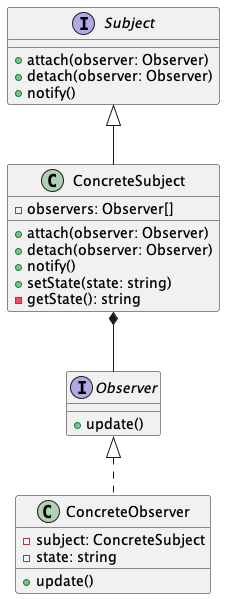
\includegraphics[width=0.25\textwidth]{fig/uml/default-observer.png}
  \caption{Einfaches Observer Pattern}
  \label{fig:default-observer}
\end{figure}

Das Observer Pattern ermöglicht eine flexible und erweiterbare Architektur, da Subjekte und Beobachter unabhängig voneinander implementiert werden können. Subjekte können Beobachter hinzufügen oder entfernen, ohne dass dies Auswirkungen auf den Rest des Systems hat. Beobachter können ebenfalls hinzugefügt oder entfernt werden, ohne dass Änderungen an anderen Teilen des Systems vorgenommen werden müssen.
\\\\
Die Abbildung~\ref{fig:default-observer} zeigt das Observer Pattern mit drei Komponenten: Subject, Observer und ConcreteSubject. Das Subject ist eine Schnittstelle, die von den Subjekten implementiert wird, die beobachtet werden sollen. Es definiert Methoden zum Hinzufügen, Entfernen und Benachrichtigen von Beobachtern. Der Observer ist eine Schnittstelle, die von allen Beobachtern implementiert wird, und definiert eine Methode zum Aktualisieren des Beobachters, wenn sich der Zustand des Subjekts ändert.

Der ConcreteSubject ist das Subjekt, das beobachtet werden soll. Es hält eine Liste von Beobachtern und implementiert die Methoden zum Hinzufügen, Entfernen und Benachrichtigen von Beobachtern. Der ConcreteObserver ist ein Beobachter, der den Zustand des Subjekts aktualisiert, wenn sich dieser ändert.
\\\\
Das Observer Pattern ermöglicht eine lose Kopplung zwischen Subjekten und Beobachtern, da Subjekte nicht von spezifischen Beobachtern abhängig sind und Beobachter nicht von spezifischen Subjekten. Man beachte, dass eine lose Kopplung zwischen den Komponenten gelingt, aber eine enge Kopplung bei der Kommunikation unterstützt wird. 
\\\\
Für unser Anwendungsbeispiel angepasst, soll das Oberver-Pattern zwischen der KundenApp (View) und der Lampe (Model) etabliert werden. Eine vereinfachte Architektur könnte wie in Abbildung~\ref{fig:mvc-observer} aufgebaut werden. 

\begin{figure}[ht]
  \centering
  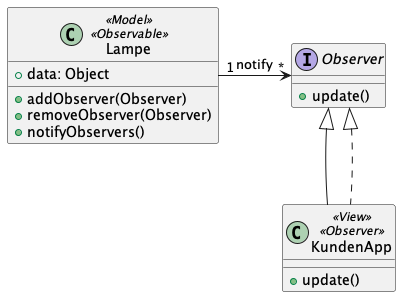
\includegraphics[width=0.45\textwidth]{fig/uml/mvc-observer.png}
  \caption{Observer Pattern als Verbindung zwischen Model und View}
  \label{fig:mvc-observer}
\end{figure}

Natürlich ist ein Architektur-Modell nicht ausreichend, um das gesamte Design zu beschreiben, auch das MVC Architektur-Modell braucht weitere Informationen für das vollständige System. Eine wichtige zusätzliche Information ist das Verhalten der Architektur. Auch für dieses Verhalten bestehen \enquote{Best Practise} Ansätze, die wir als Verhaltensmuster (Behavioral Patterns) beschreiben. 
\\\\
\textbf{Verhaltensmuster} (Behavioral Patterns) sind Entwurfsmuster in der Softwareentwicklung, die sich mit der Organisation und Steuerung von Objekten und deren Interaktionen beschäftigen. Sie beschreiben, wie verschiedene Objekte zusammenarbeiten und wie sie Verhaltensweisen und Aufgaben koordinieren.
\\\\
Behavioral Patterns beschreiben das Verhalten von Objekten in bestimmten Situationen und stellen somit Lösungen für wiederkehrende Probleme bereit, wie z.B. die Steuerung von Abläufen, die Verwaltung von Zuständen oder die Behandlung von Fehlern. Es gibt verschiedene Arten von Behavioral Patterns, die je nach Art der Aufgabe, die sie lösen sollen, in verschiedene Kategorien unterteilt werden können:
\begin{itemize}
\item \textbf{Klassifizierungsmuster} (Classification Patterns): Diese Muster beschreiben, wie Objekte in Klassen und Kategorien organisiert werden können, um eine effektive Klassifizierung und Strukturierung von Objekten zu ermöglichen. Ein Beispiel für ein solches Muster ist das Strategy Pattern.
\item \textbf{Kommunikationsmuster} (Communication Patterns): Diese Muster beschreiben, wie Objekte miteinander kommunizieren und wie Nachrichten oder Daten zwischen ihnen ausgetauscht werden können. Ein Beispiel für ein solches Muster ist das Observer Pattern.
\item \textbf{Kontrollmuster} (Control Patterns): Diese Muster beschreiben, wie Objekte kontrolliert und gesteuert werden können, um eine effektive Durchführung von Abläufen und Prozessen zu ermöglichen. Ein Beispiel für ein solches Muster ist das Command Pattern.
\item \textbf{Datenmuster} (Data Patterns): Diese Muster beschreiben, wie Daten zwischen Objekten ausgetauscht und gespeichert werden können. Ein Beispiel für ein solches Muster ist das Iterator Pattern.
\end{itemize}
Es ergibt sich natürlich, dass die Kommunikationsmuster eine besondere Bedeutung in dem Design eines verteilten Systems einnehmen. 
\\\\
Für die Beschreibung von Behavioral Patterns eignen sich in UML (Unified Modeling Language) vor allem die folgenden Diagrammtypen:
\begin{itemize}
\item \textbf{Aktivitätsdiagramme} (Activity Diagrams): Diese Diagramme werden verwendet, um die Abläufe und Prozesse in einem System oder einer Anwendung zu beschreiben. Aktivitätsdiagramme können verwendet werden, um die Interaktionen zwischen verschiedenen Objekten in einem Behavioral Pattern darzustellen.
\item \textbf{Sequenzdiagramme} (Sequence Diagrams): Diese Diagramme werden verwendet, um die Interaktionen zwischen verschiedenen Objekten in einer bestimmten Sequenz darzustellen. Sequenzdiagramme können verwendet werden, um die Kommunikationsmuster in einem Behavioral Pattern zu beschreiben.
\item Zustandsdiagramme (State Diagrams): Diese Diagramme werden verwendet, um den Zustand eines Objekts und die Übergänge zwischen verschiedenen Zuständen zu beschreiben. Zustandsdiagramme können verwendet werden, um die Kontrollmuster in einem Behavioral Pattern zu beschreiben.
\item \textbf{Interaktionsübersichtsdiagramme} (Interaction Overview Diagrams): Diese Diagramme werden verwendet, um die Interaktionen zwischen verschiedenen Objekten und deren Kommunikationsmuster in einem System oder einer Anwendung zu beschreiben. Interaktionsübersichtsdiagramme können verwendet werden, um eine Übersicht über die Interaktionen in einem Behavioral Pattern zu geben.
\end{itemize}
Durch die Verwendung dieser Diagrammtypen können Behavioral Patterns effektiv beschrieben und visualisiert werden, was zu einer verbesserten Verständlichkeit und Kommunikation der Konzepte und Strukturen innerhalb des Patterns führt.
\\\\
In dem Fallbeispiel der Lampe soll zur Verdeutlichung die einfache Sequenz des Hinzufügen eines Observers zwischen PI (Controller) und Lampe (Model) den Nutzen verdeutlichen. 

\begin{figure}[ht]
  \centering
  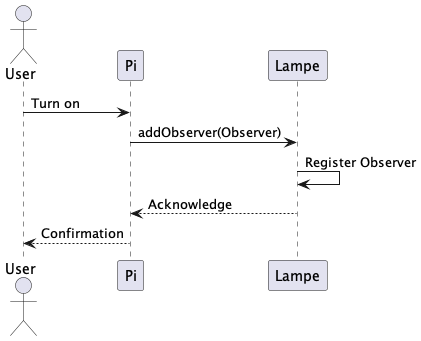
\includegraphics[width=0.55\textwidth]{fig/uml/seq-mvc-observer.png}
  \caption{Observer Pattern als Verbindung zwischen Model und View}
  \label{fig:seq-mvc-observer}
\end{figure}

Im Sequenzdiagramm~\ref{fig:seq-mvc-observer} sind die Schritte zum Hinzufügen eines Observers wie folgt beschrieben:
\begin{itemize}
\item Der Benutzer initiiert den Prozess, indem er den Controller bittet, einen neuen Observer hinzuzufügen.
\item Der Controller ruft die \enquote{addObserver()} Methode des Models auf und übergibt den Observer als Parameter.
\item Das Model registriert den neuen Observer intern, z.B. indem es ihn in einer Liste von Beobachtern speichert.
\item Nachdem der Observer erfolgreich registriert wurde, bestätigt das Model dies dem Controller.
\item Schließlich bestätigt der Controller dem Benutzer, dass der Observer erfolgreich hinzugefügt wurde.
\end{itemize}
Dieses Sequenzdiagramm zeigt die Interaktionen zwischen Benutzer, Controller, Model und Observer beim Hinzufügen eines Observers im Kontext eines MVC-Architekturmusters bei der Initialisierung des Systems. Es ist sicherlich schnell zu erkennen, das weder das Behavioral Pattern noch das Architecture Pattern alleine ausreichend Informationen bietet. Nur in gegenseitiger Ergänzung bieten sie ein vollständiges Bild. Dem geneigten Leser ist es in diesem Fall als Übung überlassen, die Architektur mit dem Observer zwischen Pi und Lampe zu beschreiben, wie das Verhalten an der Schnittstelle Lampe und KundenApp. 
\\\\
Ob das MVC-Pattern mit einer Kopplung über das Observer Pattern gelingt, ist nicht nur ein Design, sondern auch eine Technologie-abhängige Fragestellung. Das Observer Pattern verlangt die Möglichkeit einer unabhängigen uni-direktionalen Kommunikation zwischen dem Subjekt und den Beobachtern, die nur in eine Richtung erfolgt. Dies ist sowohl in einem Programmstack möglich, als auch bei der klassischen Socket-Kommunikation. Beispielhaft ist TCP ein Transportprotokoll auf Layer 4 des ISO-OSI Referenzmodells, welches als Schnittstelle über die Socket-API den Entwicklern bereitgestellt wird. Mit einem Applikations-Protokoll, das diese Eigenschaften nutzt, ist eine Umsetzung des Observer-Patterns eine gute Wahl. 
\\\\
% TODO Check spell
In klassischen Web-Applikationen, selbst wenn sie auf UDP oder TCP basieren, ist dies ohne weiteres nicht der Fall. Als Beispiel kann das HTTP Protokoll herangezogen werden, das auf Basis von TCP ein zustandloses Protokoll anbietet und zudem dem Request-Response-Cycle unterliegt. Insbesondere der Request-Response-Cycle setzt für jede Anfrage eine Antwort voraus und widerspricht der Funktionsweise des Observer Patterns.
\\\\
In der Praxis können Techniken wie WebSockets oder Long Polling verwendet werden, um eine Art Zustand und damit unabhängiger Kommunikation zwischen Subjekt und den Beobachtern zu simulieren und das Observer-Pattern zu verwenden, dennoch sind diese Lösungen nicht Teil von älteren HTTP Standards und in Teilen sehr fehleranfällig. Zur Erklärung, bei diesen Lösungen werden Verbindungen zwischen Subjekt und dem Beobachter aufrechterhalten und bei Zustandsänderungen werden die entsprechenden Beobachter benachrichtigt. Allerdings sind diese Techniken mit erhöhtem Aufwand verbunden und haben auch andere Nachteile, wie z.B. eine höhere Netzwerklast und eine höhere Komplexität in der Implementierung. 
Auch werden in unterschiedlichen HTTP Versionen unterschiedlichen \enquote{Workarounds} angeboten. So können bei HTTP2/ HTTP3 Technologien wie Server-Push Mechanismen genutzt werden, sie werden aber stark im Kontext der Sicherheit diskutiert. 
\\\\
Neben dem Observer Pattern, sieht man in Verteilten Systemen auch immer wieder das Callback Pattern eingesetzt, da es nur einfache Kommunikationsstrukturen braucht. In Situationen, in denen nur eine einzige Funktion oder ein einziges Objekt auf ein bestimmtes Ereignis reagieren muss, bietet daher das Callback-Pattern eine einfachere und leichter verständliche Implementierung.

Das Callback-Pattern ist auch nützlich, wenn es darum geht, den Programmfluss nicht zu blockieren, insbesondere bei asynchronen oder zeitintensiven Operationen. Es ermöglicht die Ausführung anderer Aufgaben, während die lang andauernde Operation im Hintergrund abläuft, und die Callback-Funktion wird aufgerufen, sobald die Operation abgeschlossen ist.

\subsubsection{Callback Pattern}
Das Callback-Pattern ist ein Verhaltensmuster in der Softwareentwicklung, bei dem eine Funktion (auch als Methode oder Prozedur bezeichnet) als Argument an eine andere Funktion übergeben wird. Diese übergebene Funktion, die als Callback-Funktion bezeichnet wird, wird zu einem späteren Zeitpunkt, oft nach Abschluss einer bestimmten Aufgabe oder einem Ereignis, vom aufrufenden Code ausgeführt. Das Callback-Pattern wird häufig verwendet, um asynchrone Programmierung, Ereignisbehandlung oder die Entkopplung von Funktionen zu ermöglichen.

\begin{figure}[!ht]
  \centering
  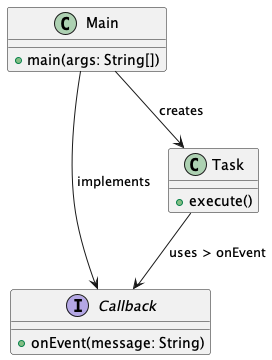
\includegraphics[width=0.30\textwidth]{fig/uml/callback-class.png}
  \caption{Callback Pattern}
  \label{fig:callback-class}
\end{figure}

Hier ist eine Beschreibung der Schlüsselelemente des Callback-Patterns:
\begin{itemize}
\item Funktion als Parameter: Im Callback-Pattern wird eine Funktion als Argument an eine andere Funktion übergeben. Die übergebene Funktion ist die Callback-Funktion.
\item Rückrufzeitpunkt: Die Callback-Funktion wird zu einem bestimmten Zeitpunkt aufgerufen, beispielsweise nach Abschluss einer Aufgabe oder beim Eintreten eines Ereignisses. Der Zeitpunkt, wann die Callback-Funktion aufgerufen wird, kann variieren und hängt von der Implementierung und den Anforderungen der Anwendung ab.
\item Entkopplung: Durch die Verwendung des Callback-Patterns können zwei Funktionen entkoppelt werden. Das bedeutet, dass die aufrufende Funktion nicht wissen muss, wie die Callback-Funktion implementiert ist, solange sie das erwartete Verhalten aufweist.
\item Einfachheit: Das Callback-Pattern ist für einfache Kommunikationsanforderungen zwischen Funktionen oder Objekten geeignet. Es ist besonders nützlich, wenn es nur eine geringe Anzahl von beteiligten Funktionen oder Objekten gibt und die Kommunikation unidirektional ist.
\item Asynchrone Programmierung: Das Callback-Pattern wird häufig in der asynchronen Programmierung verwendet, um den Programmfluss nicht zu blockieren. Wenn eine zeitintensive Operation ausgeführt wird, kann die Callback-Funktion bei Abschluss dieser Operation aufgerufen werden, sodass der restliche Code ohne Verzögerung weiterlaufen kann.
\item Ereignisgesteuert: Das Callback-Pattern eignet sich gut für ereignisgesteuerte Programmierung, bei der bestimmte Aktionen aufgrund von Ereignissen oder Benutzerinteraktionen ausgeführt werden sollen. Die Callback-Funktionen dienen als Reaktionen auf diese Ereignisse und werden ausgeführt, wenn das Ereignis eintritt.
\end{itemize}
In dem Diagrammen ~\ref{fig:callback-class} und ~\ref{fig:callback-seq} wird das Callback-Pattern über die Callback-Schnittstelle, die Task-Klasse und die Main-Klasse dargestellt. Die Callback-Schnittstelle definiert die Methode onEvent(), die später als Callback-Funktion verwendet wird. Die Task-Klasse enthält die execute()-Methode, die die Callback-Funktion aufruft, wenn eine bestimmte Aktion oder ein bestimmtes Ereignis eintritt. Schließlich erstellt die Main-Klasse sowohl ein Task-Objekt als auch eine Implementierung der Callback-Schnittstelle und stellt die Kommunikation zwischen diesen beiden Elementen her.\\\\

\noindent\begin{minipage}{\textwidth}
\begin{lstlisting}[caption={Callback Pattern},captionpos=b,label={lst:callback}]
// Callback-Interface
interface Callback {
    void onEvent(String message);
}

// Klasse, die die Callback-Funktion verwendet
class Task {
    private Callback callback;

    public Task(Callback callback) {
        this.callback = callback;
    }

    public void execute() {
        // ... fuehre einige Aktionen aus
        callback.onEvent("Task abgeschlossen");
    }
}

// Hauptklasse
public class Main {
    public static void main(String[] args) {
        Callback callback = message -> System.out.println("Callback erhalten: " + message);
        Task task = new Task(callback);
        task.execute();
    }
}
\end{lstlisting}
\end{minipage}
Obwohl Callback Pattern und Observer Pattern beide Techniken zur Implementierung von ereignisgesteuerten Kommunikationen zwischen Objekten sind, gibt es einige wichtige Unterschiede zwischen ihnen.

\begin{itemize}
\item Im Callback Pattern wird eine Funktion (Callback-Funktion) als Parameter an ein anderes Objekt oder eine Funktion übergeben.
\item Die aufgerufene Funktion oder das aufgerufene Objekt führt die übergebene Callback-Funktion unter bestimmten Bedingungen aus (z.B. nachdem eine bestimmte Aktion abgeschlossen ist).
\item Das Callback Pattern ermöglicht eine einfache, unidirektionale Kommunikation zwischen zwei Objekten oder Funktionen.
\item Das Callback Pattern eignet sich gut für einfache und direkte Kommunikationsanforderungen, bei denen nur eine geringe Anzahl von Funktionen oder Objekten beteiligt ist.
\end{itemize}
\begin{figure}[!ht]
  \centering
  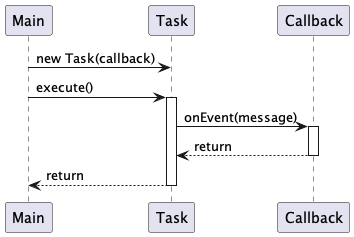
\includegraphics[width=0.50\textwidth]{fig/uml/callback-seq.png}
  \caption{Callback Pattern Sequenz}
  \label{fig:callback-seq}
\end{figure}
\begin{itemize}
\item Im Observer Pattern (auch bekannt als \enquote{Publish-Subscribe Pattern}) gibt es ein \enquote{Subject} (oder \enquote{Publisher}) und mehrere \enquote{Observer} (oder \enquote{Subscriber}). Der Code wird im Folgenden diskutiert.
\item Die Observer registrieren sich beim Subject, um über Änderungen oder Ereignisse informiert zu werden.
\item Wenn ein Ereignis beim Subject eintritt, benachrichtigt es alle registrierten Observer, indem es eine spezielle Methode in den Observer-Objekten aufruft.
\item Das Observer Pattern ermöglicht eine lose Kopplung zwischen Objekten und ist skalierbar, da eine beliebige Anzahl von Observern benachrichtigt werden kann, ohne dass das Subject deren Implementierung kennen muss.
\end{itemize}

\begin{minipage}{\textwidth}
\begin{lstlisting}[caption={Observer Pattern - ConcreteSubject},captionpos=b,label={lst:observer-I}]
import java.util.ArrayList;
import java.util.List;

// Subject-Interface
interface Subject {
    void addObserver(Observer observer);
    void removeObserver(Observer observer);
    void notifyObservers();
}

// Observer-Interface
interface Observer {
    void update(String message);
}

// ConcreteSubject
class Task implements Subject {
    private List<Observer> observers = new ArrayList<>();
    private String message;

    public void execute() {
        // ... fuehre einige Aktionen aus
        message = "Task abgeschlossen";
        notifyObservers();
    }

    @Override
    public void addObserver(Observer observer) {
        observers.add(observer);
    }

    @Override
    public void removeObserver(Observer observer) {
        observers.remove(observer);
    }

    @Override
    public void notifyObservers() {
        for (Observer observer : observers) {
                     observer.update(message);
        }
    }
}


\end{lstlisting}
\end{minipage}

Im Listing~\ref{lst:callback} und Listing~\ref{lst:observer-I},~\ref{lst:observer-II} ist zu sehen, wie das Callback Pattern und das Observer Pattern in Java-Code implementiert werden. Im Callback Pattern wird eine Funktion direkt an die ausführende Klasse (Task) übergeben, während im Observer Pattern die Observer sich beim Subject (auch Task in diesem Beispiel) registrieren, um Benachrichtigungen zu erhalten.

Für Verteilte Systeme ist sowohl für das Observer Pattern als auch das Callback Pattern die Referenzen des Callbacks bzw. des Observers eine Herausforderung. Da Verteilte Systeme sich keinen gemeinsamen Speicher teilen, muss ein Ersatz für die Adressierung der Referenz gefunden werden, dies soll zu einem späteren Zeitpunkt diskutiert werden. \\

Wenn die fehlende Adressierung gelöst ist, sollte insgesamt das Callback-Pattern in Betracht gezogen werden, wenn die Anforderungen an die Kommunikation zwischen den beteiligten Funktionen oder Objekten weniger komplex sind und eine einfachere, unidirektionale Kommunikation ausreicht. Wenn jedoch mehrere Objekte auf das gleiche Ereignis reagieren müssen oder eine losere Kopplung zwischen den beteiligten Objekten erforderlich ist, ist das Observer-Pattern besser geeignet.

Neben der Kommunikation der Komponenten, die zudem noch in eine Uni- oder Mulitcast Kommunikation unterschieden werden kann, muss auch die Initialisierung für verteilte Systeme diskutiert werden. In diesem Skript sollen neben den Singleton und den Factory Pattern auch die Initialisierung mit Dependency Injection besprochen werden.\\\\
\noindent\begin{minipage}{\textwidth}
\begin{lstlisting}[caption={Observer Pattern - Concrete Observer},captionpos=b,label={lst:observer-II}]
// ConcreteObserver
class TaskObserver implements Observer {
    private String observerName;

    public TaskObserver(String observerName) {
        this.observerName = observerName;
    }

    @Override
    public void update(String message) {
        System.out.println(observerName + " hat eine Benachrichtigung erhalten: " + message);
    }
}

// Hauptklasse
public class Main {
    public static void main(String[] args) {
        Task task = new Task();
        TaskObserver observer1 = new TaskObserver("Observer1");
        TaskObserver observer2 = new TaskObserver("Observer2");

        task.addObserver(observer1);
        task.addObserver(observer2);

        task.execute();

        task.removeObserver(observer1);

        task.execute();
    }
}
\end{lstlisting}
\end{minipage}

\subsubsection{Singleton Pattern}

Das Singleton-Pattern ist ein Entwurfsmuster, das sicherstellt, dass eine Klasse nur eine einzige Instanz hat und einen globalen Zugriffspunkt zu dieser Instanz bereitstellt. In verteilten Systemen kann die Verwendung des Singleton-Patterns einige Herausforderungen mit sich bringen, da es mehrere Knoten oder Prozesse gibt, die möglicherweise auf die Singleton-Instanz zugreifen müssen.
\begin{figure}[!ht]
  \centering
  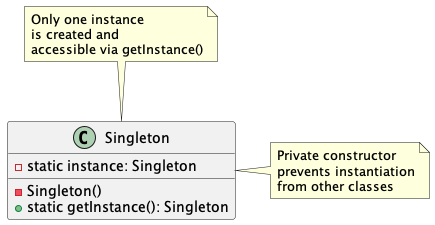
\includegraphics[width=0.45\textwidth]{fig/uml/singleton.png}
  \caption{Singleton Pattern}
  \label{fig:singleton}
\end{figure}

In dem Diagramm~\ref{fig:singleton} gibt es eine Singleton-Klasse, die das Singleton-Pattern implementiert. Die Klasse hat:
\begin{itemize}
\item Eine private statische Variable instance, die die einzige Instanz der Singleton-Klasse speichert.
\item Einen privaten Konstruktor (Singleton()), der die Erstellung von Instanzen der Singleton-Klasse von außen verhindert.
\item Eine öffentliche statische Methode getInstance(), die die einzige Instanz der Singleton-Klasse zurückgibt oder bei Bedarf erstellt.
\end{itemize}
Die Anmerkungen im Diagramm verdeutlichen, dass der private Konstruktor die Instanziierung von anderen Klassen verhindert und dass nur eine Instanz der Singleton-Klasse erstellt und über die getInstance()-Methode zugänglich gemacht wird.
\begin{itemize}
\item Ressourcenverwaltung: Das Singleton-Pattern kann bei der Verwaltung von Ressourcen, wie zum Beispiel Verbindungen zu Datenbanken oder Diensten, nützlich sein. Es kann dazu beitragen, den Ressourcenverbrauch zu minimieren, indem es verhindert, dass mehrere Verbindungen oder Instanzen erstellt werden, die dieselben Ressourcen verwenden.
\item Zentrale Steuerung: Ein Singleton kann als zentrale Steuerungs- oder Koordinationskomponente in einem verteilten System dienen, indem es sicherstellt, dass es nur eine einzige Instanz gibt, die den globalen Zustand verwaltet.
\end{itemize}
\begin{itemize}
\item Skalierbarkeit: Das Singleton-Pattern kann die Skalierbarkeit eines verteilten Systems beeinträchtigen, da alle Knoten oder Prozesse auf die einzelne Instanz des Singleton-Objekts zugreifen müssen. Dadurch kann es zu Engpässen oder Leistungsproblemen kommen, wenn die Anzahl der Knoten oder Prozesse zunimmt.
\item Synchronisation: In verteilten Systemen kann die Synchronisation von Singleton-Instanzen eine Herausforderung darstellen. Um sicherzustellen, dass alle Knoten dieselbe Singleton-Instanz verwenden, muss ein Mechanismus implementiert werden, um den globalen Zustand der Instanz konsistent zu halten. Dies kann zusätzliche Komplexität und Overhead verursachen, insbesondere wenn das verteilte System auch fehlertolerant sein muss.
\item Fehlertoleranz: Ein Singleton-Objekt kann in einem verteilten System zu einem Single Point of Failure (SPOF) werden. Wenn die Singleton-Instanz ausfällt, kann dies das gesamte System beeinträchtigen. Um dieses Problem zu umgehen, sind zusätzliche Maßnahmen wie Replikation oder Clustering erforderlich, die die Komplexität erhöhen und möglicherweise die Vorteile des Singleton-Patterns zunichte machen.
\end{itemize}
Die Eignung des Singleton-Patterns hängt in verteilten Systemen von den spezifischen Anforderungen und der Architektur des Systems ab. In einigen Fällen kann das Singleton-Pattern Vorteile bieten, wie das zentrale Verwalten von Ressourcen und die Steuerung des globalen Zustands. In anderen Fällen können die Nachteile, wie eingeschränkte Skalierbarkeit, Synchronisationsprobleme und die Notwendigkeit, Fehlertoleranz zu gewährleisten, dazu führen, dass das Singleton-Pattern für verteilte Systeme weniger geeignet ist.

\subsubsection{Factory Pattern}
Das Factory-Pattern ist ein Entwurfsmuster, das Objekterstellung auf eine separate Factory-Klasse auslagert. Dies ermöglicht die Erstellung von Objekten, ohne dass der Client-Code direkt den Konstruktor der Objekte aufrufen muss. In verteilten Systemen kann das Factory-Pattern einige Vorteile bieten:
\begin{itemize}
\item Abstraktion und Entkopplung: Das Factory-Pattern hilft, den Client-Code von den konkreten Implementierungsdetails der erstellten Objekte zu entkoppeln. In verteilten Systemen kann dies besonders nützlich sein, da Änderungen an den Implementierungen von Diensten oder Komponenten ohne Auswirkungen auf den Client-Code vorgenommen werden können. Dies erleichtert die Wartung und Skalierung des Systems.
\item Flexibilität bei der Objekterstellung: Das Factory-Pattern ermöglicht es, verschiedene Implementierungen von Objekten zu erstellen, basierend auf der Systemkonfiguration oder den Anforderungen des verteilten Systems. Dies kann dazu beitragen, dass das System einfacher an unterschiedliche Umgebungen oder Anforderungen angepasst werden kann.
\item Vereinfachung der Objekterstellung: In verteilten Systemen kann die Erstellung von Objekten, insbesondere von Ressourcen wie Verbindungen zu Datenbanken oder externen Diensten, komplex sein. Das Factory-Pattern kann dazu beitragen, diese Komplexität zu kapseln und die Erstellung von Objekten für den Client-Code zu vereinfachen. Dadurch wird der Code leichter verständlich und wartbar.
\item Zentrale Verwaltung von Ressourcen: In verteilten Systemen kann die Verwaltung von Ressourcen wie Verbindungen oder Diensten eine Herausforderung darstellen. Durch die Verwendung des Factory-Patterns können diese Ressourcen zentral erstellt und verwaltet werden, was zu einer besseren Kontrolle und einem effizienteren Ressourcenmanagement führt.
\item Load Balancing und Failover: Das Factory-Pattern kann in verteilten Systemen dazu verwendet werden, Load Balancing und Failover-Mechanismen zu implementieren. Die Factory kann die Anfragen auf verschiedene Knoten oder Instanzen verteilen, um die Last auszugleichen oder im Falle eines Ausfalls auf einen anderen Knoten umzuschalten. Dies trägt zur Skalierbarkeit und Fehlertoleranz des Systems bei.
\end{itemize}
\begin{figure}[!ht]
  \centering
  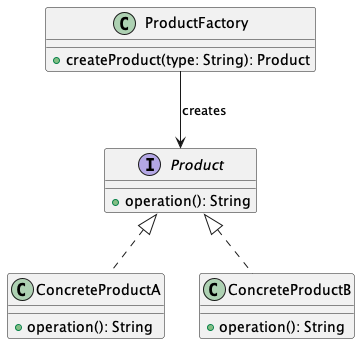
\includegraphics[width=0.45\textwidth]{fig/uml/factory-class.png}
  \caption{Factory Pattern}
  \label{fig:factory-class}
\end{figure}
Das Diagramm~\ref{fig:factory-class} beschreibt das Factory Pattern.
\begin{itemize}
\item Ein Product-Interface, das die gemeinsame Schnittstelle für alle Produkte definiert.
\item Zwei konkrete Produktklassen (ConcreteProductA und ConcreteProductB), die das Product-Interface implementieren. Sie stellen unterschiedliche Produktvarianten dar.
\item Eine ProductFactory-Klasse, die für die Erstellung von Product-Objekten verantwortlich ist.
\end{itemize}
Das Factory-Pattern kapselt die Logik zur Erstellung von Produktobjekten in der ProductFactory-Klasse. Der Client-Code verwendet die createProduct()-Methode der Factory, um ein Produktobjekt zu erstellen, ohne sich um die konkreten Implementierungsdetails der Produktklassen kümmern zu müssen. Das Diagramm zeigt, dass die ProductFactory-Klasse das Product-Interface verwendet, um Produktobjekte zu erstellen, wobei die konkreten Produktklassen die Implementierung bereitstellen.

\begin{figure}[!ht]
  \centering
  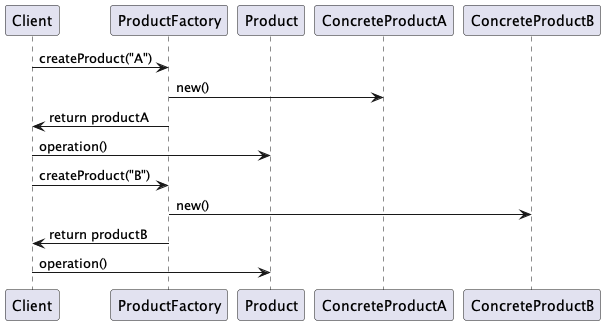
\includegraphics[width=0.85\textwidth]{fig/uml/factory-seq.png}
  \caption{Factory Pattern Sequenz}
  \label{fig:factory-seq}
\end{figure}

Insgesamt bietet das Factory-Pattern in verteilten Systemen eine Reihe von Vorteilen, die dazu beitragen, den Code sauberer und wartbarer zu gestalten, die Skalierbarkeit und Fehlertoleranz zu verbessern und die Verwaltung von Ressourcen zu optimieren. Durch die Abstraktion der Objekterstellung und die zentrale Verwaltung von Ressourcen trägt das Factory-Pattern zur Effizienz und Flexibilität in verteilten Systemen bei.

Obwohl das Factory-Pattern in vielen verteilten Systemen Vorteile bietet, gibt es auch Situationen, in denen Probleme auftreten können:
\begin{itemize}
\item Kommunikationslatenz: In verteilten Systemen kann die Kommunikation zwischen den Knoten und den Factory-Instanzen Latenz verursachen. Wenn der Factory-Code auf einem zentralen Knoten gehostet wird, kann dies zu Verzögerungen bei der Objekterstellung führen und die Gesamtleistung des Systems beeinträchtigen.
\item Synchronisation: In verteilten Systemen kann die Synchronisation der Factory-Instanzen über mehrere Knoten hinweg eine Herausforderung darstellen. Wenn der Factory-Code oder die Konfigurationsinformationen geändert werden, müssen alle Factory-Instanzen im System aktualisiert werden, um konsistent zu bleiben. Dies kann zu zusätzlicher Komplexität und möglichen Inkonsistenzen führen.
\item Single Point of Failure (SPOF): Wenn die Factory zentral verwaltet wird oder auf einem einzelnen Knoten gehostet ist, kann dies zu einem Single Point of Failure führen. Im Falle eines Ausfalls dieses Knotens oder der Factory-Instanz kann das gesamte verteilte System beeinträchtigt werden. Um dieses Risiko zu minimieren, sind möglicherweise zusätzliche Maßnahmen wie Replikation oder Clustering erforderlich.
\item Erhöhte Komplexität: Obwohl das Factory-Pattern dazu beitragen kann, die Komplexität der Objekterstellung zu reduzieren, kann es in einigen Fällen auch zusätzliche Komplexität in das verteilte System einführen. Die Implementierung von Factories, die auf verschiedenen Knoten verteilt sind, kann die Systemarchitektur und das Debugging komplexer gestalten. In solchen Fällen kann es schwieriger sein, den Überblick über den Datenfluss und die Abhängigkeiten zwischen den Knoten zu behalten.
\item Schwerer zu testen: In verteilten Systemen kann das Testen von Factory-Implementierungen aufgrund der beteiligten Knoten und der möglichen Latenz- oder Synchronisationsprobleme schwieriger sein. Die Testbarkeit von Factories und den erstellten Objekten kann in solchen Umgebungen eingeschränkt sein, was zu einer geringeren Codequalität führen kann.
\item Overhead: Die Verwendung von Factories in verteilten Systemen kann zusätzlichen Overhead verursachen, insbesondere wenn die Objekterstellung häufig stattfindet oder eine große Anzahl von Knoten beteiligt ist. In solchen Fällen kann der zusätzliche Overhead, der durch die Kommunikation zwischen den Knoten und der Factory entsteht, die Leistung des Systems beeinträchtigen.
\end{itemize}

Trotz dieser Herausforderungen und Probleme kann das Factory-Pattern eine wichtige Option in der Architektur eines verteilten Systems sein. 

\subsubsection{Dependency Injection Pattern}

Das Dependency Injection (DI) Pattern ist ein Entwurfsmuster, bei dem die Abhängigkeiten eines Objekts von außen bereitgestellt werden, anstatt dass das Objekt sie selbst erstellt. Dies kann helfen, den Code modularer, testbarer und wartbarer zu gestalten. In einem verteilten System kann das DI-Pattern folgende Vorteile bieten:
\begin{itemize}
\item Entkopplung: DI ermöglicht die Entkopplung von Komponenten in einem verteilten System. Anstatt dass eine Komponente direkt von einer anderen abhängt, werden die Abhängigkeiten injiziert, wodurch die Komponenten unabhängiger voneinander werden. Dies fördert eine saubere Trennung der Zuständigkeiten und macht das System einfacher zu warten und zu erweitern.
\item Flexibilität: Durch die Verwendung von DI können verschiedene Implementierungen einer Abhängigkeit bereitgestellt werden, ohne dass der Client-Code geändert werden muss. Dies ist besonders nützlich in verteilten Systemen, in denen verschiedene Knoten unterschiedliche Implementierungen oder Konfigurationen benötigen.
\item Testbarkeit: DI verbessert die Testbarkeit von Komponenten in verteilten Systemen, da Abhängigkeiten leicht durch Mock- oder Stub-Implementierungen ersetzt werden können. Dies ermöglicht das isolierte Testen von Komponenten, ohne dass auf externe Dienste oder Ressourcen zugegriffen werden muß.
\item Zentrale Verwaltung von Ressourcen: In verteilten Systemen kann das DI-Pattern dazu beitragen, die Erstellung und Verwaltung von Ressourcen wie Datenbankverbindungen oder externen Diensten zu zentralisieren. Dies ermöglicht eine bessere Kontrolle und ein effizienteres Ressourcenmanagement.
\item Skalierbarkeit und Fehlertoleranz: Durch die Entkopplung von Komponenten und die zentrale Verwaltung von Ressourcen kann das DI-Pattern dazu beitragen, die Skalierbarkeit und Fehlertoleranz von verteilten Systemen zu verbessern. Beispielsweise können Load-Balancing- und Failover-Mechanismen einfacher implementiert werden, wenn Abhängigkeiten zentral verwaltet und injiziert werden.
\end{itemize}

In einem verteilten System kann das Dependency Injection-Pattern wie folgt angewendet werden:
\begin{itemize}
\item Definieren Sie Schnittstellen oder abstrakte Klassen für die Abhängigkeiten, die von den Komponenten des Systems benötigt werden.
\item Implementieren Sie die konkreten Klassen, die diese Schnittstellen oder abstrakten Klassen erfüllen.
\item Verwenden Sie einen DI-Container oder ein Framework (z. B. Spring in Java), um Abhängigkeiten zu konfigurieren, zu erstellen und in die jeweiligen Komponenten zu injizieren.
\item Stellen Sie sicher, dass die Komponenten im System sich nur auf die definierten Schnittstellen oder abstrakten Klassen beziehen, anstatt direkt auf die konkreten Implementierungen zuzugreifen.
\end{itemize}    
Wenn das DI-Pattern in einem verteilten System implementiert ist, können verschiedene Knoten unterschiedliche Implementierungen oder Konfigurationen der Abhängigkeiten verwenden, ohne den Code der einzelnen Komponenten ändern zu müssen. Dies ermöglicht eine größere Flexibilität und Anpassungsfähigkeit des Systems an verschiedene Umgebungen und Anforderungen. Ein Beispiel für das Dependency Injection-Pattern in einem verteilten System könnte ein System mit mehreren Microservices sein, die über ein Netzwerk kommunizieren. Jeder Microservice hat seine eigene Aufgabe und benötigt möglicherweise Zugriff auf verschiedene externe Ressourcen oder Dienste. Anstatt dass jeder Microservice direkt auf diese Ressourcen zugreift, werden die Abhängigkeiten über DI bereitgestellt. Dies ermöglicht es, die Ressourcen zentral zu verwalten und bei Bedarf unterschiedliche Implementierungen oder Konfigurationen bereitzustellen.

Um die Funktionsweise des Patterns zu verdeutlichen, soll nochmals das Fallbeispiel mit der Lampe bemüht werden. Der Fokus liegt darauf, dass der Pi (Controller) die Lampe (Model) kontrolliert. 
\\\\
Zunächst erstellen wir eine Schnittstelle für die Abhängigkeit:\\

\noindent\begin{minipage}{\textwidth}
\begin{lstlisting}[caption={Schnittstelle für die Abhängigkeit},captionpos=b,label={lst:di-interface}]
public interface BulbService {
    void doLight();
}
\end{lstlisting}
\end{minipage}

Dann erstellen wir eine Implementierung dieser Schnittstelle:\\
\noindent\begin{minipage}{\textwidth}
\begin{lstlisting}[caption={Schnittstellenimplementierung},captionpos=b,label={lst:di-interface-implementation}]

public class Bulb implements BulbService {
    public void doLight() {
        System.out.println("Do cool Stuff");
    }
}
\end{lstlisting}
\end{minipage}

Als nächstes erstellen wir die Klasse, die die Abhängigkeit benötigt:\\
\noindent\begin{minipage}{\textwidth}
\begin{lstlisting}[caption={Dependency},captionpos=b,label={lst:di-dependency}]

public class ControllerOnPI {
    private BulbService service;
    
    public ControllerOnPI(BulbService service) {
        this.service = service;
    }
    
    public void doControl() {
        service.doLight();
    }
}
\end{lstlisting}
\end{minipage}
Hier haben wir eine Konstruktor-basierte Dependency Injection verwendet, um die Abhängigkeit von MessageService in MyApplication zu injizieren.
\\\
Schließlich können wir unser Beispiel in der Main-Methode verwenden:\\\\
\noindent\begin{minipage}{\textwidth}
\begin{lstlisting}[caption={Die DI Main},captionpos=b,label={lst:di-main}]
public class Main {
    public static void main(String[] args) {
        BulbService bulb = new Bulb();
        ControllerOnPI c = new ControllerOnPI(bulb);
        
        c.doControl();
    }
}
\end{lstlisting}
\end{minipage}

Dependency Injection (DI) ist ein nützliches Muster für die Entwicklung von Anwendungen. Es hat jedoch auch Nachteile, insbesondere in verteilten Systemen. Einer der Nachteile ist, dass DI in verteilten Systemen eine zusätzliche Komplexität einführen kann, insbesondere wenn viele verschiedene Komponenten vorhanden sind, die miteinander kommunizieren müssen. DI kann auch die Leistung beeinträchtigen, insbesondere wenn die Abhängigkeiten zwischen den Komponenten in einem verteilten System über ein Netzwerk übertragen werden müssen. Ein weiterer Nachteil von DI in verteilten Systemen ist, dass es ein Sicherheitsrisiko darstellen kann, wenn es nicht ordnungsgemäß implementiert wird. Außerdem kann DI die Skalierbarkeit beeinträchtigen, wenn die Komponenten in der Anwendung nicht ordnungsgemäß entkoppelt sind. Schließlich kann DI auch das Debugging erschweren, insbesondere wenn es viele verschiedene Komponenten gibt, die miteinander interagieren. Daher müssen diese Nachteile von Dependency Injection berücksichtigt werden, wenn sie in verteilten Systemen eingesetzt wird, um sicherzustellen, dass die Implementierung angemessen ist und die Anforderungen des Systems erfüllt.

Dependency Injection (DI) wird häufig mit einem Konzept aus der Programmierung verbunden das Reflections (Reflexion) genannt wird. In der Informatik bezieht sich Reflection (Reflexion) auf die Fähigkeit eines Computerprogramms, seine eigene Struktur und sein Verhalten zur Laufzeit zu analysieren und zu manipulieren. Diese Fähigkeit ermöglicht es einem Programm, Informationen über seine eigenen Komponenten, wie Klassen, Methoden, Attribute, etc., zu untersuchen und sogar deren Eigenschaften und Funktionalitäten zu ändern.
\\\\
Reflection wird in vielen Programmiersprachen unterstützt, z. B. in Java, C\#, Python und JavaScript. Reflexion kann in verschiedenen Szenarien nützlich sein, wie zum Beispiel:

\begin{itemize}
\item Introspektion (Selbstbeobachtung): Um Informationen über Code-Elemente, wie Klassen, Methoden und Attribute, zur Laufzeit abzurufen.
\item Dynamische Erzeugung von Objekten: Um Objekte zur Laufzeit basierend auf Informationen, die zur Laufzeit verfügbar sind, zu erzeugen.
\item Erweiterbarkeit und Plug-in-Systeme: Um dynamisch Funktionalitäten oder Erweiterungen zu einem Programm hinzuzufügen, ohne es neu kompilieren zu müssen.
\item Testautomatisierung und Mocking: Um private oder interne Methoden und Attribute während der Testphase zugänglich zu machen oder zu verändern.
\end{itemize}    
Trotz seiner Vorteile kann die Verwendung von Reflection jedoch auch Nachteile haben, wie zum Beispiel:
\begin{itemize}
\item Performance: Da Reflection zur Laufzeit arbeitet, kann es zu einer verminderten Leistung führen.
\item Sicherheit: Durch den Zugriff auf private und geschützte Code-Elemente kann die Sicherheit eines Programms beeinträchtigt werden.
\item Wartbarkeit: Der Einsatz von Reflection kann zu schwer lesbarem und schwer wartbarem Code führen, da die Beziehungen zwischen Code-Elementen nicht immer offensichtlich sind.
\end{itemize}   
Daher ist es wichtig, Reflection nur dann einzusetzen, wenn es wirklich notwendig ist, und dabei auf Best Practices und Sicherheitsaspekte zu achten.

\subsubsection{Adapter und Wrapper Pattern}

Das Adapter Pattern und das Wrapper Pattern sind beide Strukturpattern, die in verteilten Systemen verwendet werden können, um die Interoperabilität zwischen verschiedenen Komponenten zu gewährleisten. Obwohl beide Muster ähnlich sind, gibt es einige Unterschiede, die im Folgenden erläutert werden.

Das Adapter Pattern ermöglicht die Zusammenarbeit von Komponenten mit unterschiedlichen Schnittstellen, indem es eine Zwischenschicht zwischen ihnen einfügt. Das Muster definiert eine Klasse, die die Schnittstelle einer Komponente in die Schnittstelle einer anderen Komponente übersetzt, so dass sie miteinander kommunizieren können. Das Adapter Pattern kann verwendet werden, um zwei Komponenten mit unterschiedlichen Protokollen oder Datenformaten miteinander zu verbinden. Es kann auch verwendet werden, um eine bestehende Komponente an eine neue Schnittstelle anzupassen, ohne den Code der Komponente selbst zu ändern.

Das Wrapper Pattern hingegen definiert eine neue Klasse, die eine vorhandene Komponente umschließt, um ihre Schnittstelle oder ihr Verhalten zu ändern oder zu erweitern. Das Muster ermöglicht es, eine Komponente anzupassen, ohne den Code der Komponente selbst zu ändern. 

Insgesamt sind sowohl das Adapter Pattern als auch das Wrapper Pattern nützliche Muster für die Entwicklung von verteilten Systemen, da sie die Interoperabilität zwischen verschiedenen Komponenten erleichtern und die Wiederverwendbarkeit von vorhandenem Code erhöhen. Die Wahl des geeigneten Musters hängt von den spezifischen Anforderungen des Systems ab.


\subsubsection{Interceptor Pattern}
Das Interceptor Pattern ist ein Behavioral Pattern, das in verteilten Systemen eingesetzt wird, um die Kommunikation zwischen Komponenten zu steuern. Das Pattern verwendet sogenannte Interceptor- Komponenten, die die eingehenden und ausgehenden Nachrichten der Anwendung abfangen und modifizieren können.

Interceptors werden verwendet, um verschiedene Funktionen auszuführen, wie z.B. Sicherheitsüberprüfungen, Protokollierung, Leistungsüberwachung und Fehlerbehebung. Interceptors können auch verwendet werden, um die Kommunikation zwischen Komponenten zu optimieren, indem sie unerwünschte Nachrichten entfernen oder redundante Nachrichten zusammenfassen.

Das Interceptor Pattern besteht aus einer Kette von Interceptor-Komponenten, die eine eingehende oder ausgehende Nachricht abfangen und modifizieren können, bevor sie an die nächste Komponente weitergeleitet wird. Jeder Interceptor kann die Nachricht bearbeiten oder sie an den nächsten Interceptor in der Kette weitergeben.

\begin{figure}[!ht]
  \centering
  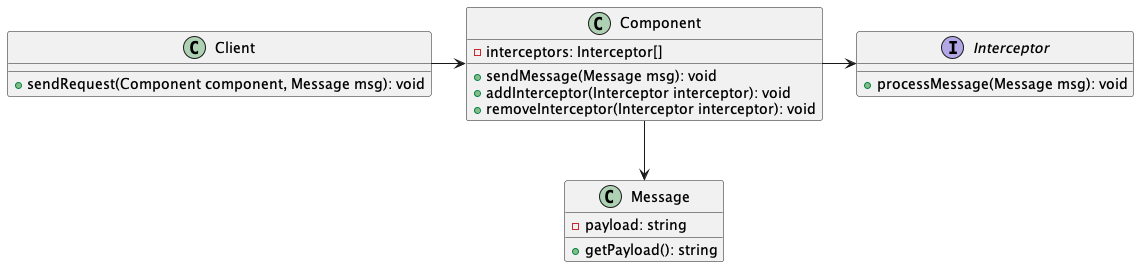
\includegraphics[width=0.99\textwidth]{fig/uml/intercept-class.png}
  \caption{Interceptor Pattern}
  \label{fig:intercept-class}
\end{figure}

Die Verwendung des Interceptor Patterns bietet mehrere Vorteile, wie z.B. die Möglichkeit, die Funktionalität einer Anwendung flexibel zu erweitern, ohne Änderungen am Quellcode der Anwendung selbst vornehmen zu müssen. Es ermöglicht auch eine effektive Steuerung der Kommunikation zwischen Komponenten und kann dazu beitragen, die Sicherheit, Leistung und Zuverlässigkeit der Anwendung zu verbessern.

\begin{figure}[!ht]
  \centering
  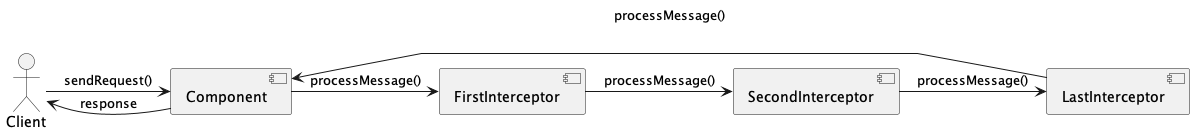
\includegraphics[width=0.99\textwidth]{fig/uml/intercept-seq.png}
  \caption{Interceptor Pattern Sequenz}
  \label{fig:intercept-seq}
\end{figure}

In diesem Beispiel~\ref{fig:intercept-seq} besteht die Component aus einer Kette von Interceptor-Komponenten (FirstInterceptor, SecondInterceptor und LastInterceptor), die die eingehenden Nachrichten abfangen und modifizieren können. Die Client-Komponente sendet eine Nachricht an die Component, die dann durch die Kette von Interceptor-Komponenten läuft, bevor sie an die Client-Komponente zurückgesendet wird.

Das Klassendiagramm~\ref{fig:intercept-class} zeigt die verschiedenen Klassen und deren Beziehungen zueinander, während das Sequenzdiagramm zeigt, wie die verschiedenen Komponenten miteinander interagieren. In beiden Diagrammen ist die Verwendung des Interceptor Patterns deutlich zu erkennen.

Insgesamt ist das Interceptor Pattern ein nützliches Pattern für die Entwicklung von verteilten Systemen, da es eine effektive Möglichkeit bietet, die Kommunikation zwischen Komponenten zu steuern und die Funktionalität der Anwendung zu erweitern.

Ein Beispiel für das Interceptor Pattern in einem verteilten System könnte wie folgt aussehen:
\\\\
Annahmen:\\
\begin{itemize}   
\item Es gibt eine Anwendung, die aus mehreren Komponenten besteht, die über ein Netzwerk miteinander kommunizieren.
\item Eine dieser Komponenten ist für die Ausführung von Finanztransaktionen verantwortlich.
\end{itemize}   
Anforderungen:
\begin{itemize}   
\item Es ist erforderlich, dass alle eingehenden und ausgehenden Finanztransaktionsnachrichten überwacht werden, um die Sicherheit und Integrität der Transaktionen zu gewährleisten.
\item Es ist auch erforderlich, dass die Leistung der Finanztransaktionen überwacht wird, um sicherzustellen, dass die Anwendung reibungslos läuft.
\end{itemize}   
Implementierung:
\begin{itemize}   
\item Das Interceptor Pattern wird eingesetzt, um eine Kette von Interceptor-Komponenten zu erstellen, die die eingehenden und ausgehenden Finanztransaktionsnachrichten abfangen und modifizieren können.
\item Der erste Interceptor in der Kette ist für die Überprüfung der Sicherheit der Finanztransaktionsnachrichten verantwortlich. Wenn die Nachricht sicherheitsrelevant ist, wird sie an den nächsten Interceptor weitergeleitet. Wenn die Nachricht jedoch als unsicher eingestuft wird, wird sie abgelehnt.
\item Der zweite Interceptor in der Kette ist für die Überwachung der Leistung der Finanztransaktionen verantwortlich. Wenn die Nachricht eine Finanztransaktion ist, wird die Leistung der Transaktion gemessen und protokolliert.
\item Der letzte Interceptor in der Kette ist für das Senden der Finanztransaktionsnachricht an die Zielkomponente verantwortlich.
\end{itemize} 
Durch die Verwendung des Interceptor Patterns können die Finanztransaktionen sicher und effektiv überwacht werden, ohne dass Änderungen am Quellcode der Anwendung selbst vorgenommen werden müssen. Die Interceptor-Komponenten können auch problemlos hinzugefügt, entfernt oder geändert werden, um den Anforderungen der Anwendung gerecht zu werden.

\subsubsection{Fassade Pattern}
Das Fassade Pattern ist ein Strukturpattern, das in verteilten Systemen verwendet werden kann, um eine vereinfachte Schnittstelle für den Zugriff auf komplexe Subsysteme bereitzustellen. Es dient als eine Art vereinfachte Schicht, die die Interaktion zwischen Client-Code und einem komplexen Subsystem abstrahiert.

In verteilten Systemen kann das Fassade Pattern genutzt werden, um die Komplexität von Systemen zu reduzieren, indem eine einzige Schnittstelle bereitgestellt wird, die als Einstiegspunkt für den Zugriff auf das System dient. Dies kann dazu beitragen, die Komplexität des Systems für den Benutzer zu reduzieren und die Wartbarkeit des Codes zu verbessern.

Das Fassade Pattern besteht aus einer Fassadenklasse, die eine vereinfachte Schnittstelle für den Zugriff auf ein komplexes Subsystem bereitstellt. Die Fassade delegiert dann die Anfragen des Clients an das Subsystem, um die gewünschten Aktionen auszuführen. Die Fassadeklasse kapselt somit das komplexe Subsystem und stellt dem Client nur eine einfachere Schnittstelle zur Verfügung.

Ein Beispiel für die Verwendung des Fassade Patterns in verteilten Systemen könnte die Verwendung einer zentralen Authentifizierungs- und Autorisierungsschicht sein. Eine Fassadenklasse könnte erstellt werden, die als Schnittstelle für den Zugriff auf diese Schicht fungiert. Die Fassadenklasse könnte dann die Anfragen des Clients an das Authentifizierungs- und Autorisierungssystem weiterleiten, um die gewünschten Aktionen auszuführen.
\\\\
In diesem Beispiel~\ref{lst:fassade} besteht das komplexe Subsystem aus den Klassen SubsystemA und SubsystemB, die jeweils eine komplexe Logik ausführen. Die Facade-Klasse ist die vereinfachte Schnittstelle für den Client und delegiert die Anfragen des Clients an das Subsystem, um die gewünschten Aktionen auszuführen. In diesem Fall führt die performAction()-Methode der Fassade einfach die Operationen von SubsystemA und SubsystemB aus.

Der Client-Code erstellt eine Instanz der Fassade und ruft die performAction()-Methode auf, um auf das komplexe Subsystem zuzugreifen. Die Fassade kapselt somit das komplexe Subsystem und stellt dem Client nur eine einfachere Schnittstelle zur Verfügung.

\noindent\begin{minipage}{\textwidth}
\begin{lstlisting}[caption={Fassade Pattern},captionpos=b,label={lst:fassade}]
// Das komplexe Subsystem
class SubsystemA {
    public void operationA() {
        // komplexe Logik
    }
}

class SubsystemB {
    public void operationB() {
        // komplexe Logik
    }
}

// Die Fassade
class Facade {
    private SubsystemA subsystemA;
    private SubsystemB subsystemB;
    
    public Facade() {
        this.subsystemA = new SubsystemA();
        this.subsystemB = new SubsystemB();
    }
    
    // Einfache Schnittstelle fuer den Client
    public void performAction() {
        subsystemA.operationA();
        subsystemB.operationB();
    }
}

// Client Code
class Client {
    public static void main(String[] args) {
        Facade facade = new Facade();
        facade.performAction();
    }
}
\end{lstlisting}
\end{minipage}


\subsubsection{Pipeline Pattern}
Das Pipeline Pattern ist ein Architekturmuster für verteilte Systeme, das es ermöglicht, komplexe Verarbeitungsprozesse aufzubauen, indem die Verarbeitung in einzelne Schritte aufgeteilt wird, die sequentiell ausgeführt werden. Jeder Schritt wird von einem spezialisierten Modul durchgeführt, das in der Lage ist, einen bestimmten Verarbeitungsschritt auszuführen.

Im Pipeline Pattern gibt es drei grundlegende Komponenten:
\begin{itemize} 
\item Die Pipeline: eine Abfolge von Verarbeitungsschritten, die in einer bestimmten Reihenfolge ausgeführt werden.
\item Die Module: spezialisierte Komponenten, die für die Durchführung jedes Verarbeitungsschritts verantwortlich sind.
\item Die Daten: die Eingabe- oder Ausgabedaten, die durch die Pipeline fließen und von den Modulen verarbeitet werden.
\end{itemize} 
Ein Beispiel für das Pipeline Pattern könnte ein System sein, das große Datenmengen verarbeiten muss. Die Daten könnten in mehrere Schritte unterteilt werden, wie z.B. das Lesen von Daten aus einer Quelle, das Filtern von Daten, das Aggregieren von Daten und das Speichern von Daten in einer Datenbank. Jeder dieser Schritte wird von einem spezialisierten Modul durchgeführt, das in der Lage ist, diesen Verarbeitungsschritt effizient auszuführen.

Das Pipeline Pattern bietet eine Vielzahl von Vorteilen für verteilte Systeme, wie z.B. eine bessere Skalierbarkeit und Flexibilität bei der Entwicklung von komplexen Verarbeitungsprozessen. Es ermöglicht auch eine bessere Wiederverwendbarkeit von Modulen und eine einfachere Wartung und Fehlerbehebung. Allerdings erfordert das Pipeline Pattern auch eine sorgfältige Planung und Gestaltung der einzelnen Verarbeitungsschritte und Module, um eine optimale Leistung und Skalierbarkeit zu gewährleisten.

\subsubsection{Watchdog}
Das Watchdog Pattern ist ein bekanntes Entwurfsmuster in der Softwareentwicklung, das zur Überwachung von Ressourcen oder Prozessen in einem System verwendet wird. Es ist besonders nützlich, um potenzielle Fehler oder Störungen frühzeitig zu erkennen und entsprechende Maßnahmen zu ergreifen, um die Stabilität und Zuverlässigkeit der Anwendung zu gewährleisten.

Im Wesentlichen besteht das Watchdog Pattern aus zwei Hauptkomponenten: dem Watchdog und dem überwachten System oder Prozess. Der Watchdog ist ein unabhängiger Prozess, der den Zustand und das Verhalten des überwachten Systems kontinuierlich überprüft. Dazu verwendet der Watchdog bestimmte Prüfkriterien oder Zeitintervalle, um festzustellen, ob das überwachte System ordnungsgemäß funktioniert oder ob es Anzeichen für Fehlfunktionen gibt.

Sollte der Watchdog feststellen, dass das überwachte System nicht mehr ordnungsgemäß funktioniert, kann er entsprechende Maßnahmen ergreifen, um das Problem zu beheben. Dies kann beispielsweise das Neustarten des fehlerhaften Prozesses, das Senden einer Benachrichtigung an einen Administrator oder das Ausführen von Fallback- oder Wiederherstellungsmechanismen sein.

Das Watchdog Pattern ist in verschiedenen Anwendungsbereichen, wie zum Beispiel eingebetteten Systemen, verteilten Systemen oder auch bei der Überwachung von Softwarekomponenten, sehr nützlich. Es hilft dabei, die Systemverfügbarkeit und -stabilität zu erhöhen und die Auswirkungen von Fehlern oder Störungen zu minimieren.

Ein wichtiger Aspekt bei der Implementierung des Watchdog Patterns ist die Trennung der Verantwortlichkeiten zwischen dem Watchdog und dem überwachten System. Der Watchdog sollte so unabhängig wie möglich vom überwachten System agieren, um sicherzustellen, dass er selbst nicht von den Problemen betroffen ist, die er überwachen soll. Dies kann beispielsweise durch die Verwendung von separaten Prozessen oder Threads erreicht werden.

Insgesamt ist das Watchdog Pattern ein leistungsfähiges Entwurfsmuster, das dazu beiträgt, die Robustheit und Zuverlässigkeit von Softwaresystemen zu erhöhen. Durch die frühzeitige Erkennung und Behebung von Problemen kann es dazu beitragen, die Ausfallzeiten und die potenziellen Auswirkungen auf Benutzer und Kunden zu reduzieren.

\subsubsection{Master-Worker Pattern}
Das Master-Worker Pattern, auch bekannt als Master-Slave Pattern, ist ein grundlegendes Entwurfsmuster in der Informatik, das speziell für verteilte Systeme entwickelt wurde. Es ist eine Methode zur Organisation von Systemen, bei der eine zentrale Einheit (Master) die Kontrolle über mehrere untergeordnete Einheiten (Worker) hat. Das Hauptziel dieses Musters ist es, die Arbeitslast effizient auf mehrere Prozessoren oder Knoten zu verteilen und die Skalierbarkeit und Zuverlässigkeit des Gesamtsystems zu verbessern.

In verteilten Systemen der Informatik ist das Master-Worker Pattern von großer Bedeutung, da es die folgenden Vorteile bietet:
\begin{itemize} 
\item Parallelisierung: Das Muster erlaubt die Aufteilung von Arbeitslasten auf mehrere Worker, wodurch Aufgaben parallel und somit schneller ausgeführt werden können. Dies ist besonders nützlich bei rechenintensiven Aufgaben und bei Systemen, bei denen Ressourcen effizient genutzt werden müssen.
\item Skalierbarkeit: Das Master-Worker Pattern ermöglicht es, einem System einfach neue Worker hinzuzufügen oder bestehende Worker zu entfernen, um die Systemleistung je nach Bedarf anzupassen. Dadurch kann das System auch bei wachsenden Anforderungen weiterhin effizient arbeiten.
\item Fehlertoleranz: Da das System aus mehreren unabhängigen Workern besteht, kann es bei einem Ausfall eines Workers immer noch weiterarbeiten. Der Master kann den ausgefallenen Worker ersetzen oder dessen Aufgaben auf andere Worker verteilen, um sicherzustellen, dass das System trotz des Ausfalls weiterhin funktioniert.
\item Vereinfachung der Anwendungsentwicklung: Das Master-Worker Pattern ermöglicht es den Entwicklern, ihre Anwendungen zu modularisieren, indem sie die Funktionalität auf verschiedene Worker aufteilen. Dadurch können Entwickler sich auf einzelne Teilaufgaben konzentrieren, was die Anwendungsentwicklung und -wartung vereinfacht.
\end{itemize}    

Ein Beispiel für die Verwendung des Master-Worker Patterns ist das MapReduce-Paradigma, das in verteilten Datenverarbeitungssystemen wie Hadoop verwendet wird. Der Master, auch als \enquote{Jobtracker} bezeichnet, teilt die Eingabedaten in kleinere Teile auf und weist diese den Workern, auch als \enquote{Tasktracker} bezeichnet, zur Verarbeitung zu. Die Worker führen ihre zugewiesenen Aufgaben aus und melden ihre Ergebnisse zurück an den Master, der diese dann zu einem einzigen Ergebnis zusammenführt.

Es wurde erstmals von Google im Jahr 2004 eingeführt und ist seitdem zu einem grundlegenden Baustein in der Verarbeitung großer Datenmengen geworden, insbesondere im Bereich des Big Data und der Datenanalyse.

MapReduce besteht aus zwei Hauptphasen: Map und Reduce.
\begin{itemize}  
\item Map-Phase: In dieser Phase werden die Eingabedaten in Key-Value-Paare aufgeteilt und anschließend parallel über die verfügbaren Knoten im Cluster verteilt. Die Map-Funktion wird auf jedem dieser Knoten ausgeführt und verarbeitet die zugeordneten Key-Value-Paare. Die Ausgabe der Map-Funktion ist eine Liste von Zwischen-Key-Value-Paaren.
\item Reduce-Phase: Die Zwischen-Key-Value-Paare aus der Map-Phase werden nach dem Schlüssel gruppiert und an die Reduce-Funktion weitergeleitet. Die Reduce-Funktion wird auf jedem Gruppenschlüssel ausgeführt und fasst die zugehörigen Werte zusammen, um die endgültigen Ergebnisse zu erzeugen.
\end{itemize}  

Ein einfaches Beispiel für das MapReduce-Paradigma ist die Wortzählung in einem Text. Angenommen, wir haben einen großen Text und möchten die Häufigkeit jedes Wortes zählen. Hier ist, wie wir dies mit MapReduce erreichen können:
\begin{itemize} 
\item Map-Phase: Zuerst wird der Text in kleinere Abschnitte aufgeteilt und auf verschiedene Knoten im Cluster verteilt. Die Map-Funktion wird auf jedem Knoten ausgeführt, um jedes Wort in den Abschnitten zu verarbeiten.

Die Map-Funktion liest die Wörter in ihrem zugewiesenen Abschnitt und erstellt ein Key-Value-Paar für jedes Wort, wobei der Schlüssel das Wort selbst ist und der Wert 1. Wenn das Wort \enquote{Hallo} beispielsweise dreimal im Abschnitt erscheint, gibt die Map-Funktion folgende Key-Value-Paare aus:

\noindent\begin{minipage}{\textwidth}
\begin{lstlisting}[caption={Ausgabe},captionpos=b,label={lst:map}]
("Hallo", 1)
("Hallo", 1)
("Hallo", 1)
\end{lstlisting}
\end{minipage}

\item Reduce-Phase: Nachdem die Map-Phase abgeschlossen ist, werden die Key-Value-Paare nach dem Schlüssel (Wort) gruppiert und an die Reduce-Funktion gesendet. In diesem Fall hätten wir eine Gruppe für das Wort \enquote{Hallo} mit den Werten [1, 1, 1].

Die Reduce-Funktion summiert die Werte für jedes Wort, um die endgültige Häufigkeit zu erhalten. Für das Wort \enquote{Hallo} würde die Reduce-Funktion die Werte addieren (1 + 1 + 1) und das endgültige Key-Value-Paar ausgeben:
\noindent\begin{minipage}{\textwidth}
\begin{lstlisting}[caption={Ausgabe},captionpos=b,label={lst:map}]
("Hallo", 3)
\end{lstlisting}
\end{minipage}
\end{itemize}  

Nachdem alle Reduce-Funktionen ausgeführt wurden, haben wir eine Liste von Key-Value-Paaren, die die Häufigkeit jedes Wortes im gesamten Text angeben.

Dieses Beispiel veranschaulicht die grundlegenden Schritte des MapReduce-Paradigmas. In der Praxis würde ein MapReduce-Framework wie Apache Hadoop diese Phasen automatisch auf einem Cluster von Computern ausführen und die Verarbeitung von großen Datenmengen ermöglichen.
